\documentclass{article}
\usepackage[utf8]{inputenc}
\usepackage{hyperref}


\usepackage{polyglossia}
\setdefaultlanguage{latvian}

\usepackage{listings}
\usepackage{color}
\usepackage{graphicx}

\definecolor{dkgreen}{rgb}{0,0.6,0}
\definecolor{gray}{rgb}{0.5,0.5,0.5}
\definecolor{mauve}{rgb}{0.58,0,0.82}

\lstset{frame=tb,
  language=Python,
  aboveskip=3mm,
  belowskip=3mm,
  showstringspaces=false,
  columns=flexible,
  basicstyle={\small\ttfamily},
  numbers=none,
  numberstyle=\tiny\color{gray},
  keywordstyle=\color{blue},
  commentstyle=\color{dkgreen},
  stringstyle=\color{mauve},
  breaklines=true,
  breakatwhitespace=true,
  tabsize=3
}



\hypersetup{
    colorlinks=true,
    linkcolor=blue,
    filecolor=blue,      
    urlcolor=blue,
}

\title{Lēts Photoshop}
\author{Marta Kalniņa, Antons Nikolajevs }
\date{Decembris 2020}

\begin{document}

\maketitle

\section{Uzdevuma nosacījumi}
Izveidot programmu ar grafisko saskarni, ar kuras palīdzību var ielasīt attēlus un ar peles kursoru iezīmēt kādu attēla apgabalu. Programma veic iezīmētās attēla daļas krāsu statistisko analīzi: parāda pikseļu gaišuma (luminosity) histogrammu un vidējo krāsu.\footnote{nosacījumi paņemti no 
 \href{https://estudijas.lu.lv/pluginfile.php/910084/mod_resource/content/2/semestra_darbi_2020.pdf}{semestra darba nosacījumu faila}}
\section{Grafiskais interfeiss}
Grafiskā interfeisa izveidei tika izmantota \href{https://kivy.org/#home}{Kivy} bibliotēka. Diemžēl logdaļas (widgets), ko piedāvā Kivy, izskatās slikti\footnote{tie izskatās tā it kā būtu veidoti, kad Windows 95 vēl bija populārs}, līdz ar to mēs pieņēmām lēmumu izmantot arī bibliotēku \href{https://github.com/kivymd/KivyMD}{KivyMD}, kas piedāvā daudz vidžetu, kas labi izskatās.

\section{Attēla apgabala iezīmēšana}
Uzdevuma nosacījumos tiek prasīts, lai lietotājs varētu iezīmēt attēla apgabalu, lai veiktu tā krāsu statistisko analīzi.
Tā kā tālākā attēla apstrāde notiek, izmantojot \textit{PIL} moduli, kur attēla koordinātas tiek skaitītas no augšējā kreisā stūra (x ass ir vērsta pa labi un y ass ir vērsta uz leju), ir nepieciešams pārveidot vienu koordinātu sistēmu uz otru. Kivy koordinātu sistēma sākas apakšējā kreisajā stūrī un x ass ir vērsta pa labi, bet y ass ir vērsta uz augšu. Visu objektu koordinātas ir objekta kreisā apakšējā stūra koordinātas. Tā kā programma piedāvā lietotājam mainīt attēla koordinātas (pārtvietot attēlu pa logu), bija nepieciešams izstrādāt algoritmu, kas pārveidos peles klikšķa koordinātas no loga koordinātu sistēmas attēla koordinātu sistēmā. Turpmāk klikšķa koordinātu apzīmēsim ar $t$, attēla koordinātu ar $i$, klikšķa koordinātu attēla koordinātu sistēmā ar $v$ un attēla izmēru logā ar $s$, bet attēla īsto izmēru ar $w$.

Acīmredzot, lai iegūtu klikšķa koordinātu attēla koordinātu sistēmā ir nepieciešams atņemt attiecīgo attēla koordinātas komponenti no klikšķa koordinātas:
$$
    v_j\prime = t_j - i_j
$$
Bet iegūtā koordināta ir koordināta attēlā ar citu izmēru, līdz at to, īsto koodinātu var atrast ar proporciju.
$$
    v_j = \frac{v_j\prime \cdot w_j}{s_j}
$$

PIL izmanto atšķirīgu no Kivy koordinātu sistēmu - koordinātu sākumpunkts atrodas augšējā kreisajā stūrī, x ass ir vērsta pa labi, bet y ass uz leju, līdz ar to koordinātu $v_j$ jāpārveido uz PIL koordinātu sistēmu, lai būtu iespējams izgriezt iezīmēto daļu.
$$
    x = w_x - v_x
$$
Bet $y = v_y$. Kodā tas tika realizēts šādi:

\begin{lstlisting}
import numpy as np
import PIL

def calculate_position(self, s_pos, e_pos, i_pos, size):
        real_start_pos = [s_pos[0] - i_pos[0], s_pos[1] - i_pos[1]]
        real_end_pos = [e_pos[0] - i_pos[0], e_pos[1] - i_pos[1]]
        img = PIL.Image.open(main_app.image_path)
        w, h = img.size
        img_pos_start = [round(w * real_start_pos[0] / size[0], 0), round(h * real_start_pos[1] / size[1], 0)]
        img_pos_end = [round(w * real_end_pos[0] / size[0], 0), round(h * real_end_pos[1] / size[1], 0)]

        _s = min((img_pos_start[0], img_pos_end[0])), h - max((img_pos_start[1], img_pos_end[1]))
        _e = max((img_pos_start[0], img_pos_end[0])), h - min((img_pos_start[1], img_pos_end[1]))
        return _s, _e
    
\end{lstlisting}

\section{Vidējās krāsas noteikšana}

Katra pikseļa krāsu nosaka trīs skaitļi no 0 līdz 255. Katrs skaitlis atbilst attiecīgās krāsas - sarkanās, zaļās un zilās (RGB) - īpatsvaram. Attēls (vai arī attēla iezīmētais apgabals), kura izmēri ir $n\times m$ pikseļi tiek glabāts kā $n\times m \times 3$ vai arī $n \times m \times 4$ (ja attēls ir RGBA\footnote{RGBA darbojas ļoti līdzīgi kā RGB, bet tam ir vēl viens papildus skaitlis no 0 līdz 255 katram pikselim, kas nosaka pikseļa caurspīdīgumu} formātā) matrica, kuru turpmāk apzīmēsim $A$ un atsevišķa pikseļa konkrētas krāsas intensitāti apzīmēsim ar $A_{ijk}$. Piemēram, pikseļa $(6, 12)$ sarkanās krāsas intensitāte ir $A_{6,12,1}$. Līdz ar to, lai noteiktu vidējo krāsu, ir jānosaka katras pamatkrāsas (sarkanās, zaļās un zilās) vidējā intensitāte. To var izdarīt šādi:
$$
    C_{k} = \frac{\sum_i^n \sum_j^m A_{i,j,k}}{n\cdot m}
$$
Sākumā var atrast vidējo vērtību katrā matricas (attēla) rindiņā $ R_{i,k} = \frac{1}{m}\sum_j^m A_{i,j,k}$, un tad no tā atrast vidējo vērtību starp rindiņu vidējām vērtībām:
$$
    C_{k} = \frac{1}{n}\sum_i^n R_{i,k}
$$
Tā kā rezultātā vispārīgā gadījumā vērtība $C_{k}$ ir daļskaitlis, tas jānoapaļo, jo tam jābūt veselam skaitlim no 0 līdz 255.

Kodā tas tika realizēts šādi:
\begin{lstlisting}
import numpy as np
import PIL

def average_color(path, start, end):
    image = PIL.Image.open(path)
    image = image.crop((*start, *end))
    average_color_per_row = np.average(image, axis=0)
    average_color = np.average(average_color_per_row, axis=0)
    
\end{lstlisting}
\section{Pikseļu gaišuma histogramma}
Lai atrastu gaišuma histogrammu, attēla apgabalu $A$ ar izmēru $n\times m\times 3$ vai $n\times m \times 4$ jāpārveido par melnbaltu attēlu, līdz ar to to var reprezentēt vienkārši kā $n\times m$ matricu. Iegūto matricu jāpārveido uz 1-d masīvu, no kura jāveido histogramma. Kodā tas tika realizēts šādi:
\begin{lstlisting}
import numpy as np
import matplotlib.pyplot as plt
import PIL

def histogram(path, start, end):
    image = PIL.Image.open(path)
    image = image.crop((*start, *end))
    image_grayscale = np.array(image.convert("L"))
    plt.hist(image_grayscale.flatten())
    plt.savefig("histogram.png")
    
\end{lstlisting}

\pagebreak
\section{Izstrādes process un piemērs}
\begin{figure}[htbp]
    \centering
    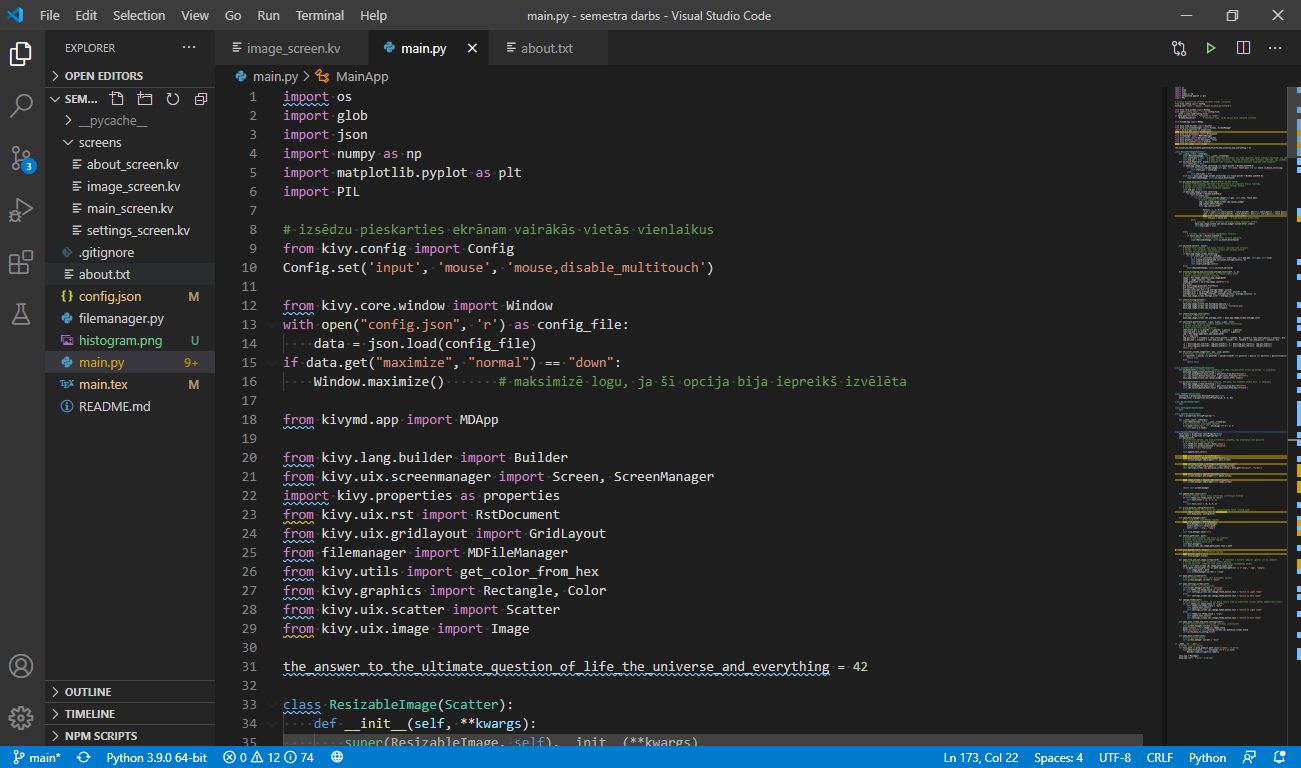
\includegraphics[width=\textwidth]{process.png}
    \caption{Programmas izstrādes process}
    \label{fig:my_label}
\end{figure}

\begin{figure}[htbp]
    \centering
    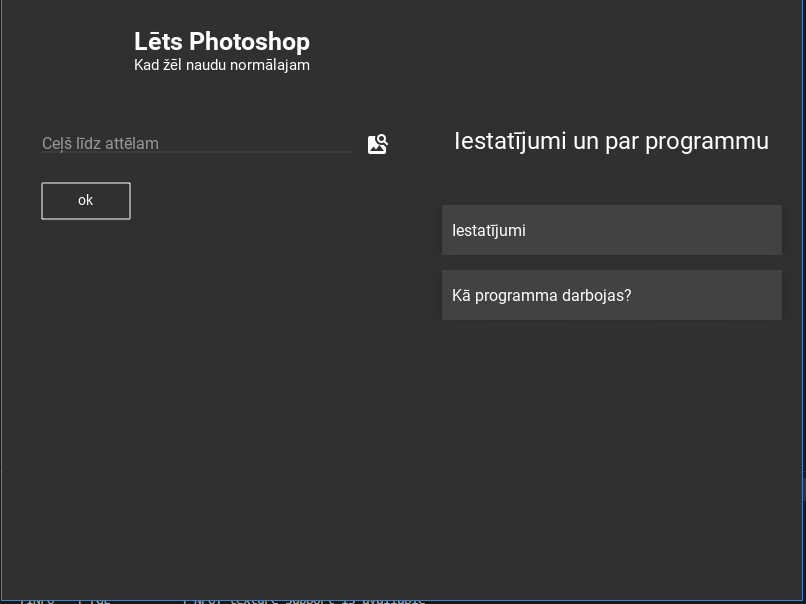
\includegraphics[width=\textwidth]{main_logs.png}
    \caption{Galvenais ekrāns, kur var izvēlēties failu}
    \label{fig:my_label}
\end{figure}

\begin{figure}[htbp]
    \centering
    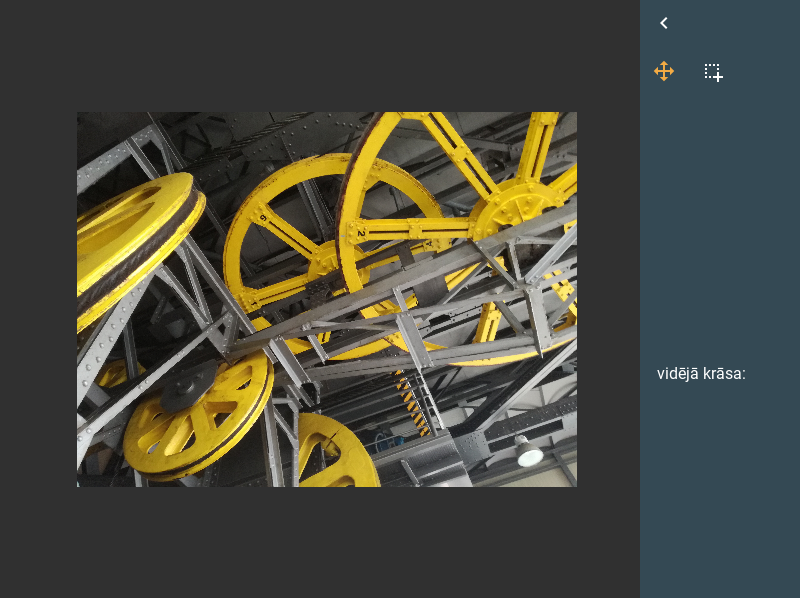
\includegraphics[width=\textwidth]{atverts_attels.png}
    \caption{Izvēlētais attēls}
    \label{fig:my_label}
\end{figure}

\begin{figure}[htbp]
    \centering
    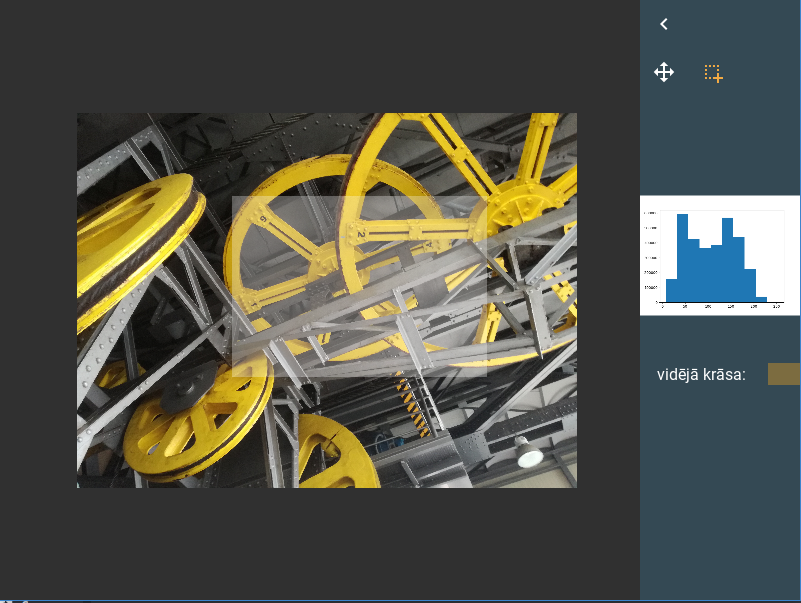
\includegraphics[width=\textwidth]{iezimets.png}
    \caption{Izvēlētā attēla apgabala iezīmēšanas process un rezultāts}
    \label{fig:my_label}
\end{figure}

\end{document}
